% vim: filetype=tex

% {{{ Latex Setup
\documentclass[12pt]{article}
\usepackage{anysize}
\usepackage[usenames]{color}
\usepackage{amsmath,amsfonts,amstext,amssymb,amsbsy,amsopn,amsthm,eucal}
\usepackage{enumitem}
\usepackage{float}
\usepackage{graphicx}
\usepackage{hyperref}
\usepackage[super,square]{natbib}
\usepackage{setspace}
\usepackage{titlesec}

\marginsize{2cm}{2cm}{1cm}{2cm}
\usepackage{soul}
\usepackage[dvipsnames]{xcolor}
\usepackage{hyperref}
\hypersetup{
    colorlinks=true,
    linkcolor=black,
    citecolor=CadetBlue,
    filecolor=CadetBlue,      
    urlcolor=CadetBlue,
}
\usepackage{multicol}
\setlength\columnsep{18pt}

\newcommand{\eqns}[1]{\begin{eqnarray*}#1\end{eqnarray*}}
\newcommand{\bmat}[1]{
    \begin{bmatrix}#1
    \end{bmatrix}
}
\newcommand{\vmat}[1]{
    \begin{vmatrix}#1
    \end{vmatrix}
}
\newcommand{\be}{\begin{enumerate}}
\newcommand{\ee}{\end{enumerate}}
\newcommand{\calL}{\mathcal{L}}
\newenvironment{solution}{\begin{trivlist}\item[]{\bf Solution:}}{\qed \end{trivlist}}

\titleformat{\section}{\normalfont\large\bfseries}{\thesection}{1em}{}
\titleformat{\subsection}{\normalfont\normalsize\bfseries}{\thesubsection}{1em}{}

% }}}

\begin{document}

\begin{center}
    \onehalfspacing
    \Large{\textbf{Characteristics of Arctic Sea Ice Meander Coefficients at Daily Frequency}}
\vspace{0.4cm}
\normalsize
\\ Alan Wang, Daniel Watkins, Monica Wilhelmus \\
\vspace{0.4cm}
\normalsize
\end{center}

\begin{multicols}{2}
\section{Introduction}
The dynamic and irregular movement of Arctic sea ice poses significant challenges 
for remote sensing analyses. While satellite imagery provides a vital means of 
observing sea ice velocity, the accuracy of straight-line velocity estimates 
diminishes over longer time intervals due to the meandering nature of ice trajectories. 
This necessitates a method to account for the deviations introduced by such nonlinear 
movement at more granular timescales.

\section{Data}
This analysis looks at the IABP Level 1 data collected from buoys placed on drifting sea ice 
as part of the buoy programme. The timestamps on buoy position data range from 2002 through 
2023. The data was cleaned using a quality control process described as follows:
\be[itemsep=-0.1cm, leftmargin=0.7cm]
    \item Fix reversed dates and positions
    \item Remove duplicated dates and positions (where both longitude and latitude stayed the 
        same between two observations)
    \item Segment the observations into groups that have gaps larger than the threshold. 
        Then, remove segments that are too short.
    \item Check for anomalous speeds between consecutive buoy positions
\ee
Afterwards, cubic spline interpolation is used to regrid the buoys to hourly time intervals within each segment.
The longitude nad latitude coordinates are converted to cartesian stereographic coordinates for analysis.

\section{Methodology}
For each buoy, we calculate the straightline hourly displacements $h_t$ where $t$ is number of hours after deployment:

$$h_t = \sqrt{(x_{t+1} - x_{t})^2 + (y_{t+1} - y_{t})^2}$$
We compute daily path distance $p_n$ by summing hourly distances for the $n$th day.
We also compute straightline daily displacement $d_n$.
Days with incomplete data are discarded.

$$p_n = \sum_{t=24n}^{24n+23}{h_t}$$
$$d_n = \sqrt{(x_{24n+24} - x_{24n})^2 + (y_{24n+24} - y_{24n})^2}$$
To quantify a buoy's deviation from it's straight line path,
we define the daily meander coefficient as the ratio of 
cumulative path length divided to net displacement in position
$$m_n = p_n/d_n$$
producing a time series at daily frequency of meander coefficients for each buoy.

As meander coefficient is relatively far removed from the original GPS data, 
we conduct sensitivity analysis to determine the uncertainty 
in meander as a function of GPS uncertainty. We assume that the buoy GPS error
be normally and independently distributed with mean $0$ and 
variance $\sigma^2$ in both the $x$ and $y$ stereographic coordinates. We
derive the uncertainty of daily path length $\sigma_p^2$ and daily displacement $\sigma_d^2$.

$$\sigma_{h_t}^2 = 2\sigma^2$$
$$\sigma_p^2 = m^2\sigma^2$$
$$\sigma_d^2 = m^2\sigma^2$$

We compiled basic summary statistics of the meander coefficient over time, and plotted 
a histogram over all regions and times. Observing that the behavior of the 
distribution was strongly defined by it's tail, we fitted lognormal, power law, and exponential distributions
to the histogram, using KS similarity to determine which was best. Further analysis 
involved plotting the autocorrelation and partial autocorrelation graphs.
\end{multicols}

\section{Results}

Based on the distribution, how do we best summarize the resulting data?

\begin{figure}[H]
    \centering
    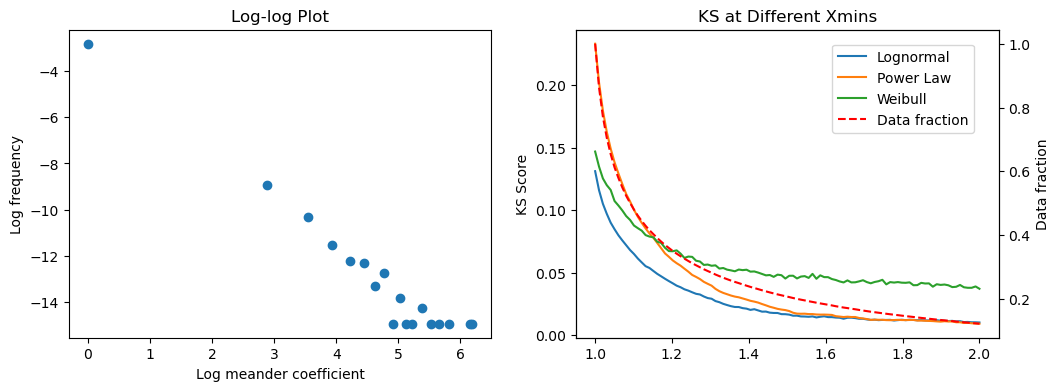
\includegraphics[width=\textwidth]{../graphs/distribution_ks.png}
    \caption{\small On the left is a log-log plot of meander coefficient frequency.
    On the right is a plot of KS-score over power law, lognormal, and Weibull distributions
    at varying xmin cutoffs.}
\end{figure}
\noindent
We observe that the distribution of the data fits better and better 
as we increase the xmin threshold. In particular, the distribution of 
meander coefficient is better modeled with a lognormal distribution at 
relatively large meander values. 


\begin{figure}[H]
    \centering
    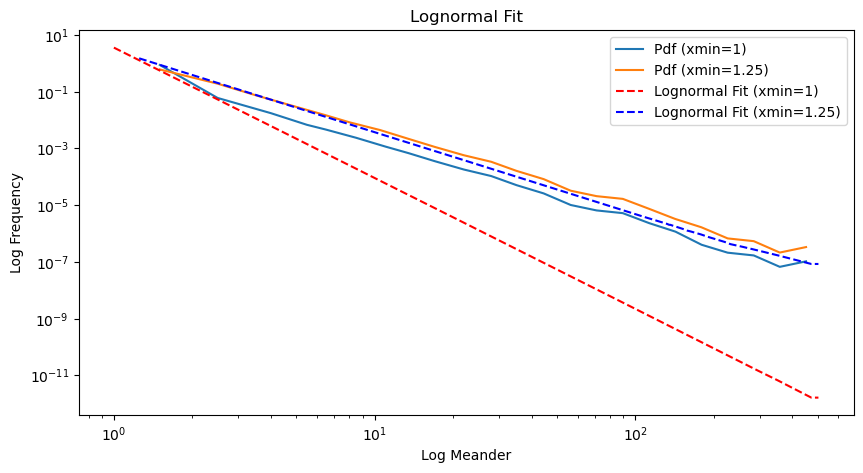
\includegraphics[width=\textwidth]{../graphs/log_normal.png}
    \caption{\small Lognormal fit pdf at xmin=$1$, containing all of the 
    data and at xmin=$1.25$, containing the upper $30\%$ of the data.}
\end{figure}

\noindent
There isn’t a universal distribution or parameterization
that works well for all levels of meander, since ice motion 
integrates velocity variability 
that itself has a variety of contributors at different time scales. 
However, the KS-plot suggests that large meanders are close to lognormal.

\begin{figure}[H]
    \centering
    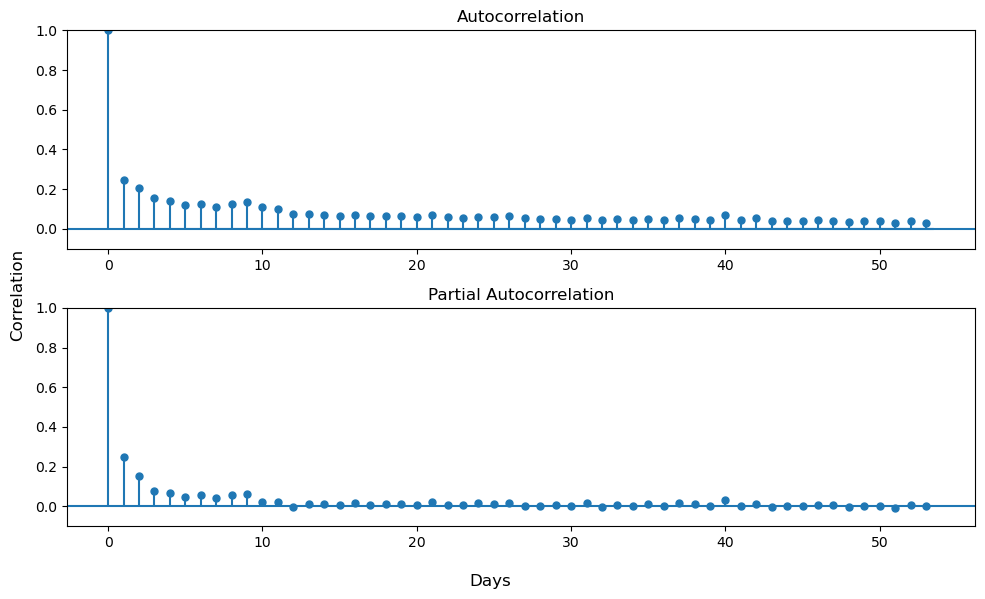
\includegraphics[width=\textwidth]{../graphs/autocorrelation.png}
    \caption{\small ACF and PACF of meander coefficient. Data from each buoy
    was concatenated before calculating autocorrelations. Buoys that contain less
    than 10 days of data were removed to reduce artifacts at longer lags.}
\end{figure}

\noindent
The ACF and PACF highlight significant autocorrelation structure in the 
meander time series.

\section{Discussion}

Further work will involve 
\be
\item Understanding the spatial variation of meander coefficient
\item Modeling meander coefficient as a stochastic process from which discrete observations are taken
\ee

\bibliographystyle{plain}
\bibliography{references}
\end{document}
